\documentclass{beamer}
\usetheme{Boadilla} 
\setbeamercovered{invisible}
\setbeamertemplate{navigation symbols}{} 
%\useoutertheme{infolines} 

\usepackage[utf8]{inputenc}
\usepackage{graphicx}

\setbeamertemplate{frametitle continuation}{} 
\usepackage{subfigure}
\usepackage{caption}
\usepackage{bm}
\usepackage{epsfig}

\usepackage{amsmath}
\usepackage{xcolor,colortbl}

\usepackage{multicol}
\usepackage{wasysym}

\usepackage{hyperref}
\usepackage{float}

\usepackage{array}
\newcolumntype{L}[1]{>{\raggedright\let\newline\\\arraybackslash\hspace{0pt}}m{#1}}
\newcolumntype{C}[1]{>{\centering\let\newline\\\arraybackslash\hspace{0pt}}m{#1}}
\newcolumntype{R}[1]{>{\raggedleft\let\newline\\\arraybackslash\hspace{0pt}}m{#1}}

\usepackage[T1]{fontenc}
\usepackage{tikz}
\usetikzlibrary{shadows}

\newcommand*\keystroke[1]{%
  \tikz[baseline=(key.base)]
    \node[%
      draw,
      fill=white,
      drop shadow={shadow xshift=0.25ex,shadow yshift=-0.25ex,fill=black,opacity=0.75},
      rectangle,
      rounded corners=2pt,
      inner sep=1pt,
      line width=0.5pt,
      font=\scriptsize\sffamily
    ](key) {#1\strut}
  ;
}

% deal with spaces in absolute paths

\usepackage[space]{grffile}
\graphicspath{{C:/Users/Yered/Dropbox/Harvard/Winter 2014/CdeC/Slides/Introduction/figures/}}

\usepackage[scaled]{helvet}
\usepackage[round]{natbib}


\begin{document}
\title[Contraste de Hipótesis]{Explorando el Transcriptoma con Datos de Expresi\'{o}n Gen\'{e}tica\\
\vspace{0.5cm}
Datos de Expresi\'{o}n Gen\'{e}tica}
\author{Yered Pita-Ju\'{a}rez}
\institute[CdeC M\'{e}rida]{}
\date{8/1/2015}


\begin{frame}
\titlepage
\end{frame}

\begin{frame}{Prueba de t}
\begin{itemize}
\item Comparar 2 grupos 
\item Determinar si las medias de dos grupos son significativamente diferentes
\end{itemize}
\begin{figure}
\centering
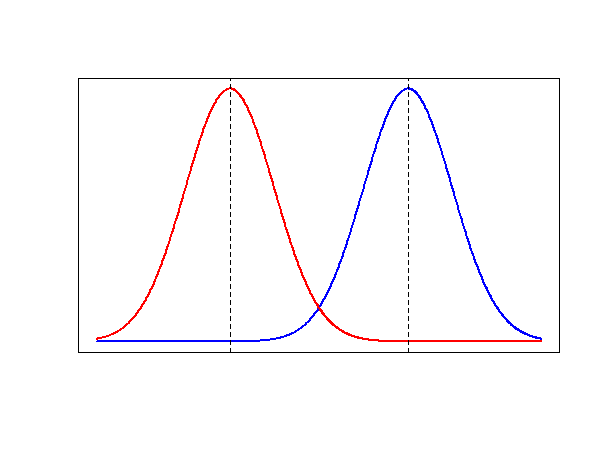
\includegraphics[scale=0.45]{t-test_diagram}
\end{figure}
\end{frame}

\begin{frame}{Prueba de t}
\begin{itemize}
\item ¿Qué tan diferentes pueden ser?
\end{itemize}
\begin{figure}
\centering
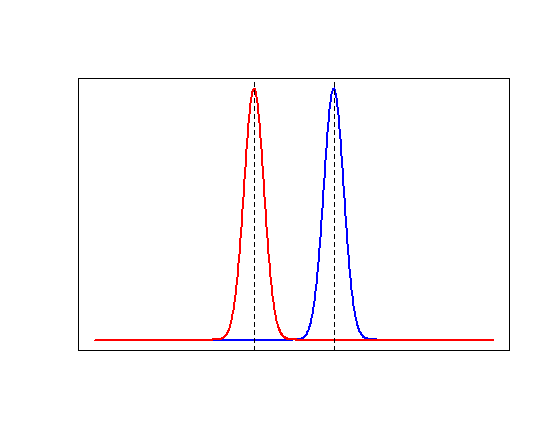
\includegraphics[scale=0.45]{t-test_lo}
\end{figure}
\end{frame}

\begin{frame}{Prueba de t}
\begin{itemize}
\item ¿Qué tan diferentes pueden ser?
\end{itemize}
\begin{figure}
\centering
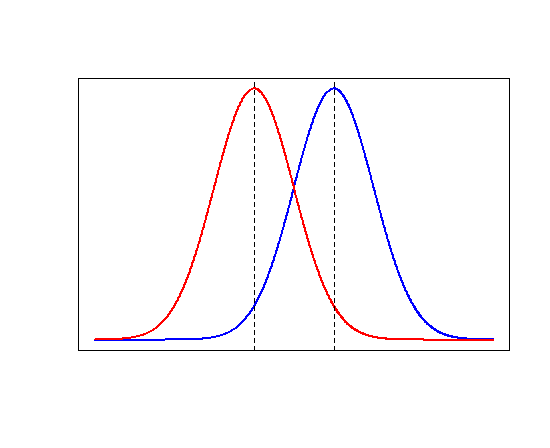
\includegraphics[scale=0.45]{t-test_med}
\end{figure}
\end{frame}

\begin{frame}{Prueba de t}
\begin{itemize}
\item ¿Qué tan diferentes pueden ser?
\end{itemize}
\begin{figure}
\centering
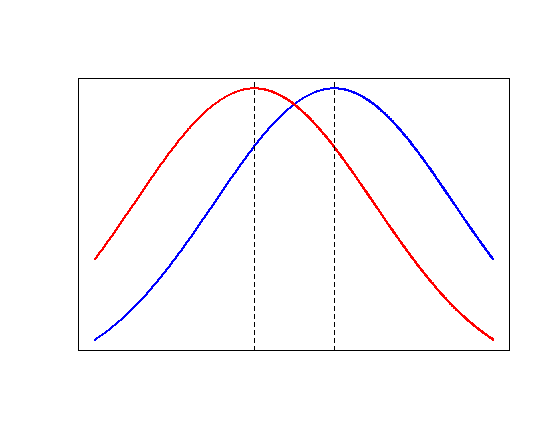
\includegraphics[scale=0.45]{t-test_hi}
\end{figure}
\end{frame}


\begin{frame}{Prueba de t}
\begin{figure}
\begin{tabular}{c}
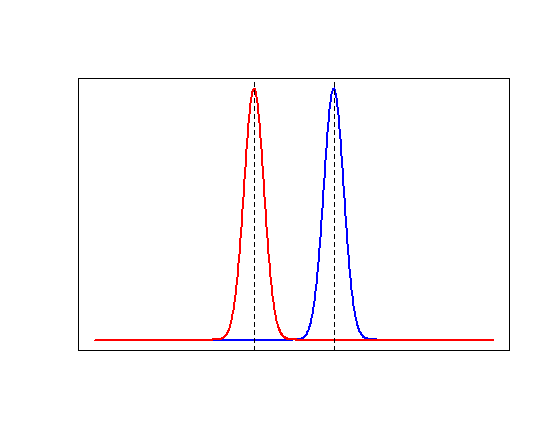
\includegraphics[width=0.27\linewidth]{t-test_lo.png} \\ 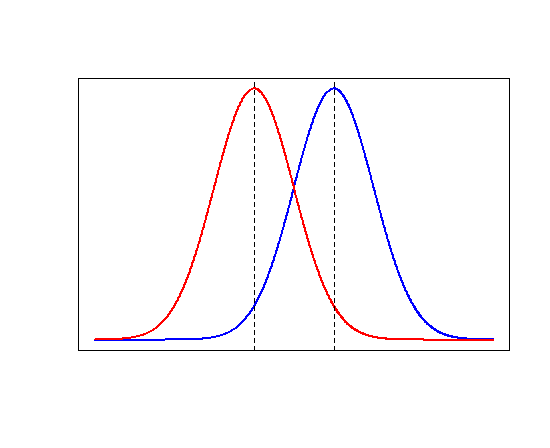
\includegraphics[width=0.27\linewidth]{t-test_med.png} \\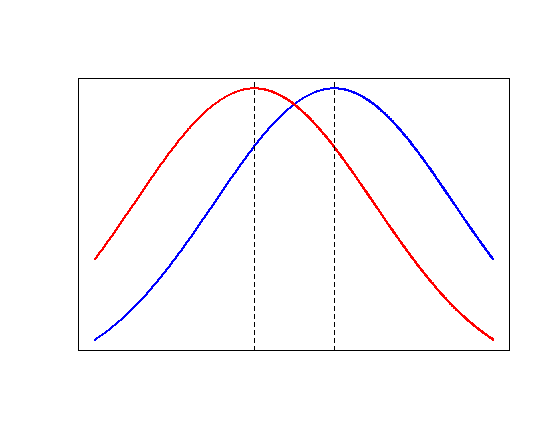
\includegraphics[width=0.27\linewidth]{t-test_hi.png} \\
\end{tabular}
\end{figure}
\end{frame}

\begin{frame}{Prueba de t}
\begin{itemize}
\item La diferencia entre las medias es la misma
\item Hay que tomar en cuenta la variabilidad de cada grupo
\item Señal: diferencia entre las medias
\item Ruido: la variabilidad de los grupos
\item estadística T
\begin{align*}
T = \dfrac{\text{señal}}{\text{ruido}} = \dfrac{\bar{X}_1-\bar{X}_2}{\text{sd}(\bar{X}_1-\bar{X}_2)}
\end{align*}
\begin{figure}
\centering
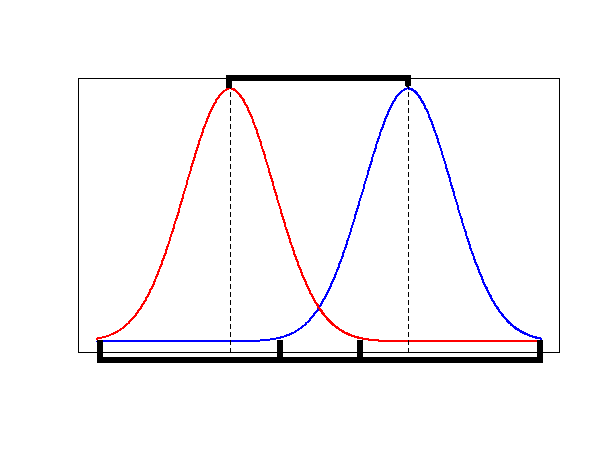
\includegraphics[scale=0.35]{t-test_diagram2.png}
\end{figure}
\end{itemize}
\end{frame}

\begin{frame}{Prueba de t}
\begin{itemize}
\item $H_0:$ las medias son iguales vs. $H_1:$ las medias son diferentes
\item $H_0:\mu_1 = \mu_2$  vs. $H_1:\mu_1 \neq \mu_2$
\item $\mu_1$ y $\mu_2$ son las medias verdaderas de los grupos
\item Solo tenemos observaciones para cada grupo
\item Estimamos las medias usando los promedios $\bar{X}_1$ y $\bar{X}_2$
\end{itemize}
\end{frame}

\begin{frame}[fragile]{Prueba de t}
\begin{itemize}
\item ¿Cómo decidimos entre $H_0$ y $H_1$?
\item Valor p: si $H_0$ es cierta, la probabilidad de observar una estadística al menos tan extrema como la observada
\item Mientras mas pequeño sea el valor p, la evidencia en contra de $H_0$ es mayor
\item Usamos el criterio $\alpha$, rechazamos $H_0$ si
\begin{align*}
p \leq \alpha
\end{align*}
\item Usualmente $\alpha=0.05$
\item En R, usa la función \verb=t.test= 
\item \texttt{t.test(x,y)} compara las medias de los vectores \verb=x= y \verb=y=
\end{itemize}
\end{frame}


\begin{frame}[fragile]
\begin{block}{Ejercicio}
\begin{itemize}
\item Usa \verb=rnorm= para generar dos vectores con la misma media y aplica la prueba de t usando \verb=t.test=
\item Usa \verb=rnorm= para generar dos vectores con medias diferentes y aplica la prueba de t usando \verb=t.test=
\end{itemize}
\end{block}
\begin{figure}[H]
\centering

\includegraphics[scale=0.15]{laptop.jpeg}
\end{figure}
\end{frame}

\begin{frame}[fragile]
\begin{block}{Ejercicio}
\begin{itemize}
\item Descarga el archivo \verb=CdeC.RDS= en tu working directory
{\small \url{https://dl.dropboxusercontent.com/u/21912429/CdeC/CdeC.RDS}}
\item Carga los datos en R usando
\begin{verbatim}
CdeC = readRDS("CdeC.RDS")
\end{verbatim}
\item \verb=CdeC= es una lista con las edades de dos clubes de ciencia
\item Calcula la edad promedio para cada club usando \verb=mean=
\item Determina si la edad promedio es significativamente diferente usando \verb=t.test=
\end{itemize}
\end{block}
%\begin{figure}[H]
%\centering
%
\includegraphics[scale=0.15]{laptop.jpeg}
%\end{figure}
\end{frame}



\begin{frame}[fragile]{Comparaciones Múltiples}
\begin{itemize}
\item Usar la prueba t para comparar muchas variables entre dos grupos
\item ¿Cuántas veces vamos a rechazar $H_0$?
\item Si usamos un valor $\alpha$ de 0.05, vamos a rechazar $H_0$ en el 5\% de los casos al azar
\item Sin ajustar los valores p nuestros resultados no son confiables
\end{itemize}
\end{frame}

\begin{frame}[fragile]{Simulación}
\begin{itemize}
\item Vamos a generar 2 vectores con la misma media usando \verb=rnorm=
\item Vamos a usar la prueba de t para comparar las medias
\item En este caso, $H_0$ siempre es cierta
\item La desición correcta es no rechazar $H_0$
\item Usando $\alpha=0.05$ vamos a estar equivocados en el 5\% de los casos 
\end{itemize}
\begin{verbatim}
sim <- function(n=10){
  x1 = rnorm(n)
  x2 = rnorm(n)
  tmp = t.test(x1,x2)
  tmp$p.value
}
res = replicate(1000,sim(n=30))
\end{verbatim}
\end{frame}

\begin{frame}[fragile]{Simulación}
\begin{verbatim}
hist(res,main="",xlab="valores p")
abline(v=0.05,col="red",lwd=2)
\end{verbatim}
\begin{figure}
\centering
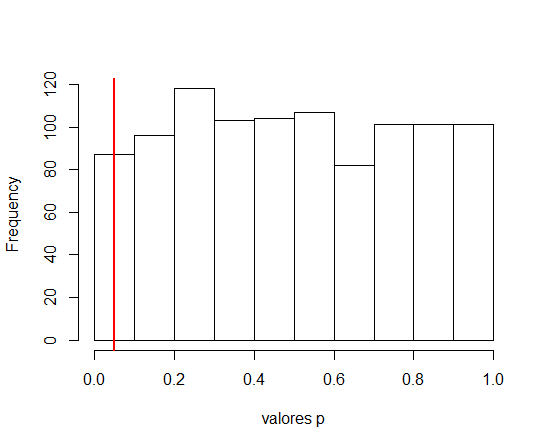
\includegraphics[scale=0.3]{sim_res00.png}
\end{figure}
\end{frame}

\begin{frame}[fragile]{Ajuste}
\begin{itemize}
\item Métodos para ajustar los valores p
\item En este caso, al ajustarlos no deberiamos tener ningun valor p menor a 0.05
\end{itemize}
\begin{verbatim}
res_adj = p.adjust(res)
hist(res_adj,xlim=c(0,1),main="",xlab="valores p ajustados")
abline(v=0.05,col="red",lwd=2)
\end{verbatim}
\begin{figure}
\centering
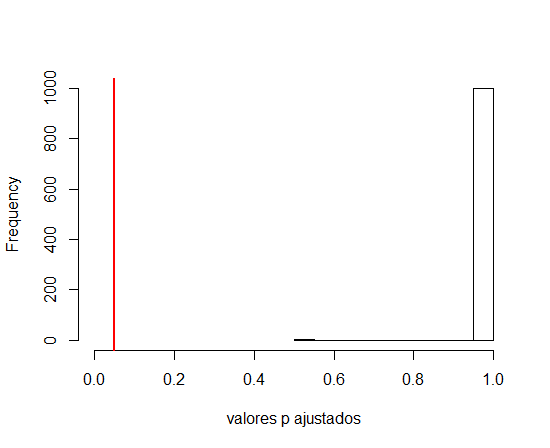
\includegraphics[scale=0.3]{sim_res01.png}
\end{figure}
\end{frame}


\end{document}

\begin{frame}[fragile]{Comparaciones Múltiples}
\end{frame}


\begin{frame}[fragile]
\begin{block}{Ejercicio}

\end{block}
\begin{figure}[H]
\centering

\includegraphics[scale=0.15]{laptop.jpeg}
\end{figure}
\end{frame}

